\documentclass[conference]{IEEEtran}
\IEEEoverridecommandlockouts
% The preceding line is only needed to identify funding in the first footnote. If that is unneeded, please comment it out.
\usepackage{cite}
\usepackage{amsmath,amssymb,amsfonts}
\usepackage{algorithmic}
\usepackage{graphicx}
\usepackage{textcomp}

% jmejia added
\usepackage[utf8]{inputenc}
\usepackage{algorithm}
\usepackage{algorithmic}
% jmejia added

\def\BibTeX{{\rm B\kern-.05em{\sc i\kern-.025em b}\kern-.08em
    T\kern-.1667em\lower.7ex\hbox{E}\kern-.125emX}}
\begin{document}

\title{Constrained Optimization with the \\Evolutionary Centers Algorithm\\
}


\author{\IEEEauthorblockN{Jes\'{u}s-Adolfo Mej\'{i}a-de-Dios and Efr\'{e}n Mezura-Montes}
\IEEEauthorblockA{\textit{Artificial Intelligence Research Center} \\
\textit{University of Veracruz}\\
Sebasti\'{a}n Camacho 5, Centro, Xalapa, Veracruz, 91000, M\'exico\\
jesusmejded@gmail.com; emezura@uv.mx}
}

\maketitle

\begin{abstract}
This paper presents the application of a new optimization algorithm based on the 
center of mass concept, called Evolutionary Centers Algorithm (ECA), to deal with 
constrained search spaces, The center of mass is adopted for creating new directions 
in the continuous search space considering the objective function values of a set 
of randomly-chosen solutions.  The selection and replacement processes are modified 
by using feasibility criteria to choose among solutions. The performance of the 
new approach is assessed by using the CEC 2017 competition benchmark for constrained 
optimization. The obtained results are compared against the competitive algorithm 
CAL-SHADE.  The results obtained are promising.
\end{abstract}

\begin{IEEEkeywords}
Constrained optimization, center of mass, evolutionary algorithm, physics-inspired algorithms 
\end{IEEEkeywords}

\section{Introduction}
Constrained optimization problems, usually found in real-world situations, are 
complex to solve due to different sources of difficulty such as highly non-linear 
objective function, large number of variables, non-linear inequality and equality 
constraints, among others \cite{Mezura11} . A numerical constrained optimization 
problem (CNOP), without loss of generality \cite{cecCop17}, can be defined as to:\\

\noindent
Minimize:
\begin{equation}
	f(\vec{x}),\ \vec{x}  \in S \subset \mathbb{R}^D
	\label{eqn:fx}
\end{equation}
%
subject to:
\begin{align*}
	g_i(\vec{x}) &\leq 0,& i =&  1 , \ldots, p \\
	h_j(\vec{x}) &= 0,& j =& p+1, \ldots, m
\end{align*}
%
where $S = \prod_{k = 1}^D  [ x_{k,\min},\ x_{k,\max} ]$ i.e. $x_k \in [ x_{k,\min},\ x_{k,\max} ]$ 
for $k = 1,2,\ldots,D$. The problem is subject to $p$ inequality constraints and 
$m - p$ equality constraints. If $\vec{x}$ satisfies $g_i( \vec{x} ) \leq 0$, for 
$i = 1, \ldots, p$ and $|h_j(\vec{x})| \leq \varepsilon$, for $j = p+1, \ldots, m$ 
with $\varepsilon > 0$ a small value; then $\vec{x}$ is regarded feasible.\\


The rest of the paper is organized as follows. A brief review of population-based 
algorithms for constrained optimization problems is presented in Section \ref{sec:related_work}. 
Section \ref{sec:eca} describes the proposal of a new metaheuristic for the solution 
of constrained optimization problems and the corresponding constraint-handling 
technique adopted. Specification of experiments and parameter setting are given 
in Section \ref{sec:experiments}. Experimental results, including a comparison 
against a recent and competitive algorithm, are presented in Section \ref{sec:results}. 
Conclusions and future work are established in Sections \ref{sec:conclusions} and 
\ref{sec:future_work}, respectively.


\section{Related Work} % (fold)
\label{sec:related_work}

Population based algorithm can be roughly classified into three main classes:
evolutionary algorithms (EAs), swarm intelligence and physics-based algorithms.
Some of the EAs are Genetic Algorithm \cite{melanie96}, Differential Evolution (DE) 
\cite{ed1995}, Evolutionary Programing (EP), Evolution Strategy (ES) and Genetic 
Programming (GP) \cite{back,spall03}.
%
One of the most popular EA for real-parameter optimization, particularly in constrained 
search spaces, is DE \cite{Mezura10}. DE was introduced by Storn and Price \cite{ed1995}  
for global optimization over continuous spaces.\\
%

Swarm intelligence (SI) groups algorithms that simulate the social behavior of 
swarms. Here, each search agent navigates using the simulated collective and social 
intelligence of creatures. Some of the most popular SI techniques for constrained 
optimization are particle swarm optimization (PSO) \cite{Mezura11}, which is inspired 
in the social behavior of birds flocks \cite{pso1995}, and the artificial bee colony 
(ABC) \cite{Mezura11}, inspired in the honey-bees foraging behavior \cite{abc2005}.\\

The third branch of metaheuristic algorithms are those based on physical metaphors. 
Some of the most popular algorithms are Gravitational  Search Algorithm (GSA) \cite{rashedi2009gsa}, 
Gravitational Local Search (GLSA) \cite{glsa}, Big-Bang Big-Crunch (BBBC) \cite{erol2006new}, 
Charged System Search (CSS) \cite{kaveh2010novel}, Central Force Optimization 
(CFO) \cite{cfo2007}, Black Hole (BH) \cite{hatamlou2013black} algorithm, and Ray 
Optimization (RO) algorithm \cite{kaveh2012new}, among others. Some recent surveys 
on this topic can be found in \cite{fisicaSurvey,biswas2013physics,xie2011convergence,DBLP:journals/corr/FisterYFBF13}. 
This kind of algorithms emulate physical systems, for example, in CFO each solution 
is a body and they move and interact through the space using gravitational force.\\
% 

As it can be noted, physics-based algorithms are gaining interest when solving 
optimization problems. However, when dealing constrained search spaces they are 
not as preferred as other approaches e.g. DE. Based on such tendency, this paper 
proposes a new approach based on the concept of center of mass, called Evolutionary 
Centers Algorithm (ECA) to solve CNOPs. A constraint-handling technique based on 
simple rules is added to ECA so as to consider feasibility information in the 
search bias. 

The following section describes our algorithm by detailing the sources of inspiration 
to propose the main variation operator within ECA. 
% section related_work (end)

\section{Evolutionary Centers Algorithm} % (fold)
\label{sec:eca}

Our approach is based on the center of mass definition, which is adopted for 
creating new directions and generate a bias in the population, and such bias is 
based on the objective function values of the solutions in the population. The 
selection criteria are modified to consider feasibility of solutions. Therefore, 
the aim of the algorithm will be generating solutions within the feasible region 
of the search space but with competitive objective function values.

%
%
\subsection{Motivation} % (fold)
The motivation of ECA is two-fold: (1) the meaning of the center of mass, and (2) 
the way EAs, swarm intelligence and other physics-based algorithms generate new 
solutions in the search space. 
% 
\begin{enumerate}
	\item The center of mass is a geometric property of any body. From a particular 
		  point of view, it is the average location of the weight of an object. 
		  In fact, it is possible to describe the motion of an object through 
		  space, based on the movement of its center of mass from one particular 
		  place to another. In such way, the population can be moved to places 
		  where the center of mass is maximized. 
	% 
	\item The way population-based approaches, like most of those mentioned in 
		  Section \ref{sec:related_work}, generate new solutions is based on 
		  Equation \ref{eqn:xxv}, where $\vec{x}_{i + 1}$ is the new solution 
		  generated by the current solution $\vec{x}_{i}$ and some update 
		  information $\vec{v}_{i + 1}$. 
\end{enumerate}
\begin{equation}
	\vec{x}_{i + 1} = \vec{x}_{i} + \vec{v}_{i + 1}
	\label{eqn:xxv}
\end{equation}
% 

Formally, the center of mass is the unique point $\vec{c}$ at the center of a 
distribution of mass $U = \{\vec{u}_1,\; \vec{u}_2 , \ldots , \vec{u}_K \}$ in a 
space with the the property that the weighted sum of position vectors relative 
to this point is zero \cite{kleppner73,serway}, as shown in Equation \ref{eq:masscenter}:
%
%
\begin{equation}
	\sum_{i = 1}^K m(\vec{u}_i) (\vec{u}_i - \vec{c}) = 0, \text{ implies } 
	%%%%%%%%%%%%%%%%%%%%%
	\vec{c} = \dfrac{1}{M} \sum_{i = 1}^K  m(\vec{u}_i)  \vec{u}_i,
	\label{eq:masscenter}
\end{equation}
%
%
where $m(\vec{u}_i)$ is the mass of $\vec{u}_i$ and  $M$ is the sum of the 
masses of vectors in $U$, and $m$ is a non-negative function.\\


For ECA, the objective function value of a given solution represents
its mass, then each solution in the population has a mass value associated,  i.e., 
we set $f(\vec{x}) = m(\vec{x})$ for all $\mathbb{R}^D$. Without loss of generality, 
it is assumed the maximization of a non-negative function $f$.




\subsection{Variation Operator} % (fold)
\label{sub:algorithm_description}

The variation operator used in ECA, inspired in the center of mass, works as follows: 
for each solution $\vec{x}_i $ in the population $P = \{ \vec{x}_1, \vec{x}_2, \ldots, \vec{x}_{N} \} $ of $N$ 
solutions, a subset $U \subset P $ with $K$ solutions is randomly chosen. After 
that, from $U$ the center of mass $\vec{c}$ is computed; then based on  a solution 
chosen at random $\vec{u}_r \in U$, a stepsize $\eta$, and the already generated 
center of mass $\vec{c}$, a search direction to locate a new solution $ \vec{y}_i$ 
is calculated. Such process is summarized in Equation \ref{eqn:vcu}:

\begin{equation}
	\vec{y}_i = \vec{x}_i + \eta ( \vec{c}_i - \vec{u}_{r} ),
	\label{eqn:vcu}
\end{equation}
%
where 
%
\begin{equation}
	\vec{c}_i = \dfrac{1} {W} \sum_{u \in U} f(\vec{u}) \cdot \vec{u} , 
			\hspace{0.5cm} 
			W = \sum_{ \vec{u} \in U} f(\vec{u}).
	\label{eqn:center}
\end{equation}

It is worth mentioning that the variation operator in Equation \ref{eqn:vcu} 
provides a bias to the most promising solutions, but also considers the position 
of the other solutions in $U$, as depicted in  Figure \ref{fig:masses}. 

\begin{figure}[!ht]
	\centering
	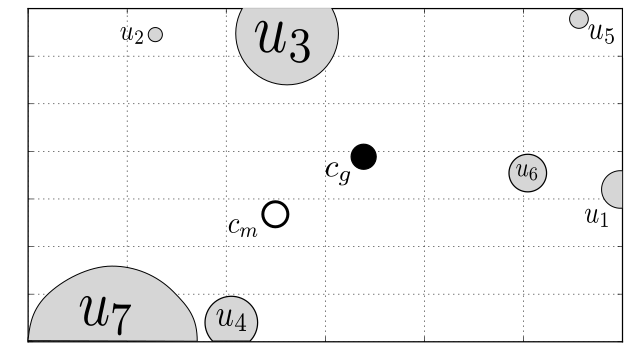
\includegraphics[width=7cm]{img/masses.pdf}
	\caption{$c_m$ is center of mass, $c_g$ is geometric center of gray points. %
	Gray point radius is its mass. Note the bias given by the weighted sum.}
	\label{fig:masses}       % Give a unique label
\end{figure}
%
%
The bias is precisely given by Equation (\ref{eqn:center}) because for a solution 
with the highest mass, the position of the center of mass is near  
its position. It is then important to remark that this bias is constraint-independent, i.e., 
no feasibility information is used in the variation operator. 
%

\subsection{Constraint-Handling} % (fold)
\label{sec:constraint_handling}

Initialization with feasible solutions is a very time consuming process and, in 
some cases, it is almost impossible to produce a feasible solution randomly 
\cite{castillofoundations}, CH-ECA (Constraint-Handling ECA) does not consider 
the initial population to be feasible. In contrast, a set of feasibility rules 
are adopted as criteria when choosing between the current solution $\vec{x}$ and 
the new one generated by the center of mass operator $\vec{y}$ and also when adding 
new solutions for the replacement process (detailed in the next subsection). 
Considering that the new solution $\vec{y}$ is preferred over the current solution 
$\vec{x}$ the conditions in Equation \ref{eqn:rules} must hold:

\begin{equation}
	\begin{cases}
	\overline{\nu}( \vec{y} ) < \overline{\nu}( \vec{x} )  \text{ or}\\
	% 
	\overline{\nu}( \vec{y} ) = \overline{\nu}( \vec{x} ) \text{ and } f(\vec{y}) > f(\vec{x})
		% 
	\end{cases}
	\label{eqn:rules}
\end{equation}
where $\overline{\nu}$ is the mean value of all constraints' violations defined as:

\begin{equation}
	\overline{\nu}( \vec{x} ) = \dfrac{1}{m} \left[ \sum_{i=1}^q G_i(\vec{x}) + \sum_{j=q+1}^m H_i(\vec{x}) \right],
	\label{eqn:nu}
\end{equation}
%
with 
\begin{eqnarray}
	G_i(\vec{x}) &=&
	\begin{cases}
		g_i(\vec{x})   & g_i(\vec{x}) > 0,  \\
		    0          & g_i(\vec{x}) \leq 0,
	\end{cases}
	\\
	%
	H_i(\vec{x}) &=&
	\begin{cases}
		|h_i(\vec{x})|   & |h_i(\vec{x})| - \varepsilon  > 0,  \\
		    0            & |h_j(\vec{x})| - \varepsilon \leq 0
	\end{cases}
	.
	%
\end{eqnarray}
%
Note that, $G_i(\vec{x})$ and $H_i(\vec{x})$ are zero when the solution is feasible. 
Also, they are non-negative functions. Here, according to \cite{cecCop17}, we set 
tolerance $\varepsilon = 0.0001$ and $g_i(\vec{x}) \leq 0,\ h_j(\vec{x}) = 0$ are 
$m$ constraints.\\


\subsection{Population Replacement} % (fold)

Let $P$ and $A$  be  non-empty sets of individuals. The former is the current 
population and the latter is the set of new solutions generated by the CH-ECA 
variation operator, which were better than their corresponding solutions based 
on the criteria defined in Equation \ref{eqn:rules}. 

To promote a low selection pressure, the solutions in $P$ are shuffled and then 
binary tournaments based on the rules in Equation \ref{eqn:rules} are carried out 
between each solution in $P$ and the corresponding solution in $A$. The winners 
are located in the population for the next generation. Based on this type of 
replacement and the selection process between current and new solution described 
in the previous subsection CH-ECA is adapted to solve CNOPs. 

\begin{figure}[!ht]
	\centering
	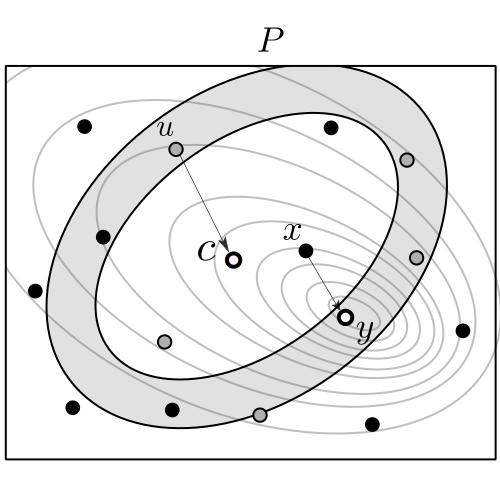
\includegraphics[width=5cm]{img/ecaG.pdf}
	\caption{Schematic diagram representing a generation of CH-ECA. Gray points % 
	represent elements in $U$. Gray area is representing the feasible region.}
	\label{fig:ecag}       % Give a unique label
\end{figure}


\subsection{CH-ECA}

CH-ECA pseudocode is detailed in Algorithm \ref{alg:ch.eca} and a scheme of its 
operation is shown in Figure \ref{fig:ecag}. CH-ECA has only two parameters: the 
number of neighbors $K$ and  the maximum stepsize $\eta_{\max}$. 

\begin{algorithm}[!ht]
	\caption{CH-ECA Algorithm}
	\label{alg:ch.eca}
	\begin{algorithmic}[1]
 		\renewcommand{\algorithmicrequire}{\textbf{Input:}}
 		\renewcommand{\algorithmicensure}{\textbf{Output:}}
		\REQUIRE {$K = 7, \; \eta_{\max} = 2$}
		%\State poplulation size = 20 $\times$ dimension
		\STATE $N \gets 2K * D$
		\STATE Generate and evaluate start population $P$ with $N$ elements
		\STATE { Evaluate $g_i$ and $h_j$ constraints}
		\WHILE{the end criterion is not achieved}
			\STATE $A = \emptyset$
			\FOR {each $\vec{x}$ in $P$}
				\STATE Generate $U \subset P$ such that  card$(U) = K$
				\STATE Calculate $\vec{c}$ using $U$ with (\ref{eqn:center})
				\STATE $\eta \gets \text{rand}(0,\; \eta_{\max}) $ 
				\STATE $\vec{y} \gets \vec{x} + \eta  * (\vec{c} - \vec{u}) $ 
						where $ \vec{u} \in U $ random
				
				\IF{ $\vec{y}$ is better than $\vec{x}$ using rules in Equation \ref{eqn:rules}}
					\STATE Append $\vec{y} $ in $A$
				\ENDIF
			\ENDFOR
			\STATE {   $P \gets $ best elements in $P \cup A$ based on binary 
					   tournaments and Equation \ref{eqn:rules} %
					}
		\ENDWHILE
		\RETURN { best solution} in $P$
		% \EndProcedure
	\end{algorithmic}
\end{algorithm}

% section constraint_handling (end)

\section{Experiments} % (fold)
\label{sec:experiments}

In order to evaluate the performance of CH-ECA, we used a set of twenty eight 
benchmark problems of the 2017 CEC competition on constrained single objective 
real-parameter optimization, which can be found in \cite{cecCop17}. This set 
includes different types of objective functions and constraints, e.g., separable, 
non-separable and rotated. Equality and inequality constraints are considered as well.\\

According to the above mentioned benchmark \cite{cecCop17}, the termination criterion 
for the algorithm is the maximum function evaluations MAXFES$=20000 \times D$, where 
$D$ is the dimensionality of the test problem. Based on the same reference \cite{cecCop17}, 25
independent runs of the proposed algorithm were recorded on the 28 test problem 
for $D = 10, 30, 50$ and $100$, with the same CH-ECA parameter values (obtained 
by preliminary tests) for all experiments as follows:

\begin{itemize}
	\item Inputs: $K = 7$, $\eta_{\max} = 2$. 
	\item Population size: $N = 2K * D$.
	\item Stop Condition: when MAXFES are reached.
	\item $\eta$ in step 9 in Algorithm \ref{alg:ch.eca} is a uniform random 
		  number between $(0,\ \eta_{\max} ]$.
\end{itemize}

% section experiments (end)



\section{Results} % (fold)
\label{sec:results}

The statistical results (best, worst, mean, and standard deviation values) obtained 
by CH-ECA in 25 independent runs are accompanied by the feasibility rate (FR) 
which is defined as \textit{(\# of feasible runs) / Total runs}, where a feasible 
run is a run where at least one feasible solution was found in MAXFES.\\
% 

Tables \ref{tab:d10}, \ref{tab:d30}, \ref{tab:d50} and \ref{tab:d100} include the 
CH-ECA results for dimensions 10, 30, 50 and 100, respectively. It is worth noting 
that CH-ECA was able to find feasible solutions in twenty two 10D, twenty one 30D, 
fourteen 50D and ten 100D test problems, out of twenty eight. Furthermore, in most 
cases the standard deviation values are low, showing CH-ECA robustness in different 
types of constrained search spaces.\\
% 

\begin{table}[!]
	\caption{CH-ECA statistical results and feasibility rate (FR) in$10D$ test problems. ``--'' means no feasible solutions found.}
	% 
	\centering
	\begin{tabular}{|c|c|c|c|c|c|c|}
	\hline
     & Best & Worst & Mean & Std. & FR \\ \hline \hline
C01 & 0.000E+00 & 0.000E+00 & 0.000E+00 & 0.000E+00 &  100 \\ 
C02 & 0.000E+00 & 0.000E+00 & 0.000E+00 & 0.000E+00 &  100 \\ 
C03 & 0.000E+00 & 0.000E+00 & 0.000E+00 & 0.000E+00 &  100 \\ 
C04 & 1.691E+01 & 1.691E+01 & 2.894E+01 & 6.935E+00 &  100 \\ 
C05 & 0.000E+00 & 0.000E+00 & 0.000E+00 & 0.000E+00 &  100 \\ 
C06 & 6.965E+00 & 6.965E+00 & 1.421E+01 & 5.669E+00 &  100 \\ 
C07 &  -- &  -- &  -- &  -- &    0 \\ 
C08 &  -- &  -- &  -- &  -- &    0 \\ 
C09 & 2.851E+00 & 2.851E+00 & 5.916E+00 & 2.431E+00 &   32 \\ 
C10 &  -- &  -- &  -- &  -- &    0 \\ 
C11 &  -- &  -- &  -- &  -- &    0 \\ 
C12 & 0.000E+00 & 0.000E+00 & 8.988E--01 & 1.556E+00 &  100 \\ 
C13 & 0.000E+00 & 0.000E+00 & 4.784E--01 & 1.322E+00 &  100 \\ 
C14 & 0.000E+00 & 0.000E+00 & 0.000E+00 & 0.000E+00 &  100 \\ 
C15 & -9.999E+00 & -9.999E+00 & -5.381E+00 & 2.641E+00 &  100 \\ 
C16 & 6.432E+09 & 6.432E+09 & 6.593E+09 & 1.050E+08 &   80 \\ 
C17 & 0.000E+00 & 0.000E+00 & 0.000E+00 & 0.000E+00 &  100 \\ 
C18 & 0.000E+00 & 0.000E+00 & 7.147E+00 & 1.598E+01 &   20 \\ 
C19 &  -- &  -- &  -- &  -- &    0 \\ 
C20 & 2.715E+00 & 2.715E+00 & 2.888E+00 & 6.640E--02 &  100 \\ 
C21 & 0.000E+00 & 0.000E+00 & 8.175E--01 & 1.380E+00 &  100 \\ 
C22 & 0.000E+00 & 0.000E+00 & 6.379E--01 & 1.492E+00 &  100 \\ 
C23 & 0.000E+00 & 0.000E+00 & 0.000E+00 & 0.000E+00 &  100 \\ 
C24 & -1.000E+01 & -1.000E+01 & -6.833E+00 & 3.087E+00 &  100 \\ 
C25 & 5.906E+08 & 5.906E+08 & 5.906E+08 & 0.000E+00 &  100 \\ 
C26 & 0.000E+00 & 0.000E+00 & 0.000E+00 & 0.000E+00 &  100 \\ 
C27 & 0.000E+00 & 0.000E+00 & 5.786E+00 & 9.881E+00 &   28 \\ 
C28 &  -- &  -- &  -- &  -- &    0 \\ 
\hline
	\end{tabular}
	\label{tab:d10}
\end{table}
% 
% 
% 
\begin{table}[!]
	\caption{CH-ECA statistical results and feasibility rate (FR) in$30D$ test problems. ``--'' means no feasible solutions found.}
	% 
	\centering
	%
	\begin{tabular}{|c|c|c|c|c|c|c|}
	\hline
     & Best & Worst & Mean & Std. & FR \\ \hline \hline
C01 & 3.204E--08 & 3.204E--08 & 4.167E--06 & 1.090E--05 &  100 \\ 
C02 & 0.000E+00 & 0.000E+00 & 2.285E--05 & 1.024E--04 &  100 \\ 
C03 & 1.889E--07 & 1.889E--07 & 1.871E--05 & 3.904E--05 &  100 \\ 
C04 & 1.086E+02 & 1.086E+02 & 1.543E+02 & 4.942E+01 &  100 \\ 
C05 & 1.219E+01 & 1.219E+01 & 2.363E+01 & 1.265E+01 &  100 \\ 
C06 & 9.400E+01 & 9.400E+01 & 1.532E+02 & 4.291E+01 &  100 \\ 
C07 &  -- &  -- &  -- &  -- &    0 \\ 
C08 &  -- &  -- &  -- &  -- &    0 \\ 
C09 & 7.430E+00 & 7.430E+00 & 1.108E+01 & 4.812E+00 &   20 \\ 
C10 &  -- &  -- &  -- &  -- &    0 \\ 
C11 &  -- &  -- &  -- &  -- &    0 \\ 
C12 & 5.450E+00 & 5.450E+00 & 1.124E+01 & 7.533E+00 &  100 \\ 
C13 & 1.284E+04 & 1.284E+04 & 3.496E+04 & 1.713E+04 &   48 \\ 
C14 & 7.419E--05 & 7.419E--05 & 6.191E--01 & 5.670E--01 &  100 \\ 
C15 & -3.927E+00 & -3.927E+00 & 8.496E--01 & 3.285E+00 &  100 \\ 
C16 & 3.823E+10 & 3.823E+10 & 3.894E+10 & 4.687E+08 &  100 \\ 
C17 & 7.607E--07 & 7.607E--07 & 1.301E--01 & 1.705E--01 &  100 \\ 
C18 & 2.025E+01 & 2.025E+01 & 3.923E+01 & 2.685E+01 &    8 \\ 
C19 &  -- &  -- &  -- &  -- &    0 \\ 
C20 & 1.133E+01 & 1.133E+01 & 1.159E+01 & 1.475E--01 &  100 \\ 
C21 & 6.404E+00 & 6.404E+00 & 1.353E+01 & 1.029E+01 &  100 \\ 
C22 & 2.616E+04 & 2.616E+04 & 5.120E+04 & 2.044E+04 &   24 \\ 
C23 & 2.141E--04 & 2.141E--04 & 4.647E--01 & 5.912E--01 &  100 \\ 
C24 & -3.927E+00 & -3.927E+00 & 2.105E+00 & 2.856E+00 &  100 \\ 
C25 &  -- &  -- &  -- &  -- &    0 \\ 
C26 & 1.156E--06 & 1.156E--06 & 1.073E--01 & 1.746E--01 &  100 \\ 
C27 & 2.025E+01 & 2.025E+01 & 3.216E+01 & 1.406E+01 &   16 \\ 
C28 &  -- &  -- &  -- &  -- &    0 \\ 
\hline
	\end{tabular}
	\label{tab:d30}
\end{table}
% 
% 
% 
\begin{table}[!]
	\caption{CH-ECA statistical results and feasibility rate (FR) in$50D$ test problems. ``--'' means no feasible solutions found.}
	% 
	\centering
	%
	\begin{tabular}{|c|c|c|c|c|c|c|}
	\hline
     & Best & Worst & Mean & Std. & FR \\ \hline \hline
C01 & 4.914E+01 & 4.914E+01 & 2.660E+02 & 1.941E+02 &  100 \\ 
C02 & 2.645E+01 & 2.645E+01 & 2.080E+02 & 1.326E+02 &  100 \\ 
C03 & 1.827E+02 & 1.827E+02 & 7.052E+02 & 3.771E+02 &  100 \\ 
C04 & 2.008E+02 & 2.008E+02 & 2.990E+02 & 4.828E+01 &  100 \\ 
C05 & 8.247E+01 & 8.247E+01 & 1.912E+02 & 7.258E+01 &  100 \\ 
C06 & 2.817E+02 & 2.817E+02 & 4.674E+02 & 1.096E+02 &  100 \\ 
C07 &  -- &  -- &  -- &  -- &    0 \\ 
C08 &  -- &  -- &  -- &  -- &    0 \\ 
C09 & 6.711E+00 & 6.711E+00 & 1.081E+01 & 2.946E+00 &   36 \\ 
C10 &  -- &  -- &  -- &  -- &    0 \\ 
C11 &  -- &  -- &  -- &  -- &    0 \\ 
C12 &  -- &  -- &  -- &  -- &    0 \\ 
C13 &  -- &  -- &  -- &  -- &    0 \\ 
C14 &  -- &  -- &  -- &  -- &    0 \\ 
C15 & 2.356E+00 & 2.356E+00 & 6.629E+00 & 2.991E+00 &  100 \\ 
C16 & 7.558E+10 & 7.558E+10 & 7.641E+10 & 6.619E+08 &  100 \\ 
C17 & 7.229E--01 & 7.229E--01 & 9.250E--01 & 1.002E--01 &   76 \\ 
C18 &  -- &  -- &  -- &  -- &    0 \\ 
C19 &  -- &  -- &  -- &  -- &    0 \\ 
C20 & 2.036E+01 & 2.036E+01 & 2.067E+01 & 1.931E--01 &  100 \\ 
C21 &  -- &  -- &  -- &  -- &    0 \\ 
C22 &  -- &  -- &  -- &  -- &    0 \\ 
C23 &  -- &  -- &  -- &  -- &    0 \\ 
C24 & 2.356E+00 & 2.356E+00 & 9.142E+00 & 3.591E+00 &  100 \\ 
C25 & 1.925E+09 & 1.925E+09 & 1.925E+09 & 0.000E+00 &  100 \\ 
C26 & 9.131E--01 & 9.131E--01 & 9.807E--01 & 4.522E--02 &   16 \\ 
C27 &  -- &  -- &  -- &  -- &    0 \\ 
C28 &  -- &  -- &  -- &  -- &    0 \\ 
\hline
	\end{tabular}
	\label{tab:d50}
\end{table}
% 
% 
% 
\begin{table}[!]
	\caption{CH-ECA statistical results and feasibility rate (FR) in$100D$ test problems. ``--'' means no feasible solutions found.}
	% 
	\centering
	%
	\begin{tabular}{|c|c|c|c|c|c|c|}
	\hline
     & Best & Worst & Mean & Std. & FR \\ \hline \hline
C01 & 4.989E+03 & 4.989E+03 & 8.793E+03 & 2.057E+03 &  100 \\ 
C02 & 2.969E+03 & 2.969E+03 & 4.915E+03 & 1.300E+03 &  100 \\ 
C03 & 5.570E+03 & 5.570E+03 & 9.405E+03 & 1.963E+03 &  100 \\ 
C04 & 6.627E+02 & 6.627E+02 & 8.400E+02 & 1.464E+02 &  100 \\ 
C05 & 3.068E+03 & 3.068E+03 & 6.806E+03 & 2.636E+03 &  100 \\ 
C06 & 1.147E+03 & 1.147E+03 & 1.494E+03 & 1.980E+02 &  100 \\ 
C07 &  -- &  -- &  -- &  -- &    0 \\ 
C08 &  -- &  -- &  -- &  -- &    0 \\ 
C09 &  -- &  -- &  -- &  -- &    0 \\ 
C10 &  -- &  -- &  -- &  -- &    0 \\ 
C11 &  -- &  -- &  -- &  -- &    0 \\ 
C12 &  -- &  -- &  -- &  -- &    0 \\ 
C13 &  -- &  -- &  -- &  -- &    0 \\ 
C14 &  -- &  -- &  -- &  -- &    0 \\ 
C15 & 8.639E+00 & 8.639E+00 & 1.442E+01 & 1.740E+00 &  100 \\ 
C16 & 9.061E+10 & 9.061E+10 & 9.184E+10 & 6.868E+08 &  100 \\ 
C17 &  -- &  -- &  -- &  -- &    0 \\ 
C18 &  -- &  -- &  -- &  -- &    0 \\ 
C19 &  -- &  -- &  -- &  -- &    0 \\ 
C20 & 4.384E+01 & 4.384E+01 & 4.418E+01 & 1.906E--01 &  100 \\ 
C21 &  -- &  -- &  -- &  -- &    0 \\ 
C22 &  -- &  -- &  -- &  -- &    0 \\ 
C23 &  -- &  -- &  -- &  -- &    0 \\ 
C24 & 1.492E+01 & 1.492E+01 & 2.225E+01 & 4.730E+00 &   24 \\ 
C25 &  -- &  -- &  -- &  -- &    0 \\ 
C26 &  -- &  -- &  -- &  -- &    0 \\ 
C27 &  -- &  -- &  -- &  -- &    0 \\ 
C28 &  -- &  -- &  -- &  -- &    0 \\ 
\hline
	\end{tabular}
	\label{tab:d100}
\end{table}







To enhance our experiments, we compared CH-ECA against a  competitive algorithm 
in the CEC 2017 competition on constrained real-parameter single-objective 
optimization (CAL-SHADE) \cite{zamuda2017adaptive}, which is an adaptive algorithm 
based on differential evolution. The comparison, based on 25 independent runs by 
each algorithm, is presented in Tables \ref{tab:d10c}, \ref{tab:d30c}, \ref{tab:d50c} 
and \ref{tab:d100c} for dimension 10, 30, 50 and 100, respectively. In such Tables, 
the last column contains a ``$\approx$'', ``--'' or ``+'' symbol. ``+'' means that 
CH-ECA outperformed CAL-SHADE in the function  	in the corresponding row, ``-'' 
means that CAL-SHADE outperformed CH-ECA, and  ``$\approx$'' means that no difference 
was observed between algorithms. Here, ``algorithm $\mathcal{A}_1$ outperforms 
algorithm $\mathcal{A}_2$'' means FR$_{\mathcal{A}_1} > $ FR$_{\mathcal{A}_2}$ 
or (FR$_{\mathcal{A}_1} = $ FR$_{\mathcal{A}_2}) \wedge ($ Mean$_{A_1} < $ Mean$_{A_2}$). 
This is a simplified ranking method based on \cite{cecCop17}. \\

As we can see in Table \ref{tab:d10c} for 10D test problems, CH-ECA outperformed 
CAL-SHADE in eighteen test functions, it reached similar results in four test 
problems and it was outperformed by CAL-SHADE in six of them. As a summary for 
10D, CH-ECA was competitive in twenty two test problems, out of twenty eight. %
%
Regarding 30D, Table \ref{tab:d30c} shows that our approach was able to outperform 
CAL-SHADE in twelve test functions, while CAL-SHADE was better in fourteen test 
problems, and no differences were observed in two test problems. The overall 
performance in 30D indicates CH-ECA being competitive in 14 test problems, out 
of twenty eight. 
%
In Table \ref{tab:d50c}, where 50D problems are considered, CH-ECA provided better 
results in eight problems, CAL-SHADE was superior in sixteen and in four problems 
no differences were observed. Based on those results, CH-ECA was competitive in 
twelve 50D test problems, out of twenty eight. 

Finally, for 100D test problems in Table \ref{tab:d100c}, CH-ECA was better in 
five functions, CAL-SHADE was better in tirtheen and no differences were observed 
in ten problems. As a result, CH-ECA was competitive in fifteen 100D test problems, 
out of twenty eight. The overall comparison is summarized in Table \ref{tab:summary}.


\begin{table}[!]
	\caption{CH-ECA and CAL-SHADE statistical values and feasibility rates (FR) for $10D$ problems. ``--'' means no feasible solutions found.}
	% 
	\centering
	%
	\begin{tabular}{|c|r|r|c|c|c|}
	 \hline
	 &\multicolumn{2}{|c|}{Mean} & \multicolumn{2}{|c|}{FR} & \\
	\cline{2-5}
	    & CH-ECA & CAL-SHADE & CH-ECA & CAL-SHADE & \\ \hline
C01 & 0.000E+00 & 0.000E+00 &  100 &  100 & $\approx$ \\ 
C02 & 0.000E+00 & 0.000E+00 &  100 &  100 & $\approx$ \\ 
C03 & 0.000E+00 & 1.100E+05 &  100 &   44 & + \\ 
C04 & 2.894E+01 & 3.874E+01 &  100 &  100 & + \\ 
C05 & 0.000E+00 & 9.568E--01 &  100 &  100 & + \\ 
C06 & 1.421E+01 & 5.496E+02 &  100 &   96 & + \\ 
C07 &  -- & -4.874E+01 &    0 &   68 & -- \\ 
C08 &  -- & -1.348E--03 &    0 &  100 & -- \\ 
C09 & 5.916E+00 & 1.255E--01 &   32 &  100 & -- \\ 
C10 &  -- & -5.100E--04 &    0 &  100 & -- \\ 
C11 &  -- & -1.563E--01 &    0 &  100 & -- \\ 
C12 & 8.988E--01 & 3.988E+00 &  100 &  100 & + \\ 
C13 & 4.784E--01 & 1.116E+00 &  100 &  100 & + \\ 
C14 & 0.000E+00 & 2.641E+00 &  100 &  100 & + \\ 
C15 & -5.381E+00 & 1.625E+01 &  100 &   68 & + \\ 
C16 & 6.593E+09 & 6.542E+01 &   80 &   60 & + \\ 
C17 & 0.000E+00 &  -- &  100 &    0 & + \\ 
C18 & 7.147E+00 &  -- &   20 &    0 & + \\ 
C19 &  -- &  -- &    0 &    0 & $\approx$ \\ 
C20 & 2.888E+00 & 8.686E--01 &  100 &  100 & -- \\ 
C21 & 8.175E--01 & 6.863E+00 &  100 &  100 & + \\ 
C22 & 6.379E--01 & 6.668E+00 &  100 &  100 & + \\ 
C23 & 0.000E+00 & 2.528E+00 &  100 &  100 & + \\ 
C24 & -6.833E+00 & 1.574E+01 &  100 &   40 & + \\ 
C25 & 5.906E+08 & 6.114E+01 &  100 &   60 & + \\ 
C26 & 0.000E+00 &  -- &  100 &    0 & + \\ 
C27 & 5.786E+00 &  -- &   28 &    0 & + \\ 
C28 &  -- &  -- &    0 &    0 & $\approx$ \\ 
   \hline
	\end{tabular}
	\label{tab:d10c}
\end{table}

% 
% 
% 
\begin{table}[!]
	\caption{CH-ECA and CAL-SHADE statistical values and feasibility rates (FR) for $30D$ problems. ``--'' means no feasible solutions found.}
	% 
	\centering
	%
	\begin{tabular}{|c|r|r|c|c|c|}
	 \hline
	 &\multicolumn{2}{|c|}{Mean} & \multicolumn{2}{|c|}{FR} & \\
	\cline{2-5}
	 & CH-ECA & CAL-SHADE & CH-ECA & CAL-SHADE & \\ \hline

C01 & 4.167E--06 & 0.000E+00 &  100 &  100 & -- \\ 
C02 & 2.285E--05 & 0.000E+00 &  100 &  100 & -- \\ 
C03 & 1.871E--05 & 1.299E+06 &  100 &   32 & + \\ 
C04 & 1.543E+02 & 1.157E+02 &  100 &  100 & -- \\ 
C05 & 2.363E+01 & 7.973E--01 &  100 &  100 & -- \\ 
C06 & 1.532E+02 & 3.745E+03 &  100 &  100 & + \\ 
C07 &  -- & -2.412E+01 &    0 &   52 & -- \\ 
C08 &  -- & -2.840E--04 &    0 &  100 & -- \\ 
C09 & 1.108E+01 & 2.336E--02 &   20 &   96 & -- \\ 
C10 &  -- & -1.030E--04 &    0 &  100 & -- \\ 
C11 &  -- & 7.808E--01 &    0 &  100 & -- \\ 
C12 & 1.124E+01 & 1.423E+01 &  100 &  100 & + \\ 
C13 & 3.496E+04 & 3.535E+03 &   48 &  100 & -- \\ 
C14 & 6.191E--01 & 1.548E+00 &  100 &  100 & + \\ 
C15 & 8.496E--01 & 2.405E+01 &  100 &   48 & + \\ 
C16 & 3.894E+10 & 2.119E+02 &  100 &   16 & + \\ 
C17 & 1.301E--01 &  -- &  100 &    0 & + \\ 
C18 & 3.923E+01 &  -- &    8 &    0 & + \\ 
C19 &  -- &  -- &    0 &    0 & $\approx$ \\ 
C20 & 1.159E+01 & 2.113E+00 &  100 &  100 & -- \\ 
C21 & 1.353E+01 & 1.326E+01 &  100 &  100 & -- \\ 
C22 & 5.120E+04 & 3.421E+04 &   24 &   72 & -- \\ 
C23 & 4.647E--01 & 1.582E+00 &  100 &   84 & + \\ 
C24 & 2.105E+00 & 2.088E+01 &  100 &   20 & + \\ 
C25 &  -- & 2.072E+02 &    0 &   32 & -- \\ 
C26 & 1.073E--01 &  -- &  100 &    0 & + \\ 
C27 & 3.216E+01 &  -- &   16 &    0 & + \\ 
C28 &  -- &  -- &    0 &    0 & $\approx$ \\ 
   \hline
	\end{tabular}
	\label{tab:d30c}
\end{table}
% 
% 
% 
\begin{table}[!]
	\caption{CH-ECA and CAL-SHADE statistical values and feasibility rates (FR) for $50D$ problems. ``--'' means no feasible solutions found.}
	% 
	\centering
	%
	\begin{tabular}{|c|r|r|c|c|c|}
	 \hline
	 &\multicolumn{2}{|c|}{Mean} & \multicolumn{2}{|c|}{FR} & \\
	\cline{2-5}
	 & CH-ECA & CAL-SHADE & CH-ECA & CAL-SHADE & \\ \hline

C01 & 2.660E+02 & 0.000E+00 &  100 &  100 & -- \\ 
C02 & 2.080E+02 & 0.000E+00 &  100 &  100 & -- \\ 
C03 & 7.052E+02 & 6.641E+06 &  100 &   48 & + \\ 
C04 & 2.990E+02 & 1.874E+02 &  100 &  100 & -- \\ 
C05 & 1.912E+02 & 3.189E--01 &  100 &  100 & -- \\ 
C06 & 4.674E+02 & 6.365E+03 &  100 &  100 & + \\ 
C07 &  -- & -6.811E+01 &    0 &   56 & -- \\ 
C08 &  -- & 9.928E--04 &    0 &  100 & -- \\ 
C09 & 1.081E+01 & 8.100E--02 &   36 &   84 & -- \\ 
C10 &  -- & -4.284E--05 &    0 &  100 & -- \\ 
C11 &  -- & 4.758E+00 &    0 &   20 & -- \\ 
C12 &  -- & 2.476E+01 &    0 &  100 & -- \\ 
C13 &  -- & 2.866E+04 &    0 &   88 & -- \\ 
C14 &  -- & 1.229E+00 &    0 &  100 & -- \\ 
C15 & 6.629E+00 & 3.049E+01 &  100 &   12 & + \\ 
C16 & 7.641E+10 & 3.470E+02 &  100 &   12 & + \\ 
C17 & 9.250E--01 &  -- &   76 &    0 & + \\ 
C18 &  -- &  -- &    0 &    0 & $\approx$ \\ 
C19 &  -- &  -- &    0 &    0 & $\approx$ \\ 
C20 & 2.067E+01 & 3.619E+00 &  100 &  100 & -- \\ 
C21 &  -- & 1.266E+01 &    0 &  100 & -- \\ 
C22 &  -- & 6.176E+04 &    0 &   36 & -- \\ 
C23 &  -- & 1.145E+00 &    0 &   84 & -- \\ 
C24 & 9.142E+00 & 2.090E+01 &  100 &   28 & + \\ 
C25 & 1.925E+09 & 3.540E+02 &  100 &   32 & + \\ 
C26 & 9.807E--01 &  -- &   16 &    0 & + \\ 
C27 &  -- &  -- &    0 &    0 & $\approx$ \\ 
C28 &  -- &  -- &    0 &    0 & $\approx$ \\ 
   \hline
	\end{tabular}
	\label{tab:d50c}
\end{table}
% 
% 
% 
\begin{table}[!]
	\caption{CH-ECA and CAL-SHADE statistical values and feasibility rates (FR) for $100D$ problems. ``--'' means no feasible solutions found.}
	% 
	\centering
	%
	\begin{tabular}{|c|r|r|c|c|c|}
	 \hline
	 &\multicolumn{2}{|c|}{Mean} & \multicolumn{2}{|c|}{FR} & \\
	\cline{2-5}
	 & CH-ECA & CAL-SHADE & CH-ECA & CAL-SHADE & \\ \hline

C01 & 8.793E+03 & 9.777E--01 &  100 &  100 & -- \\ 
C02 & 4.915E+03 & 3.661E--01 &  100 &  100 & -- \\ 
C03 & 9.405E+03 & 1.514E+07 &  100 &   16 & + \\ 
C04 & 8.400E+02 & 4.136E+02 &  100 &  100 & -- \\ 
C05 & 6.806E+03 & 8.188E--01 &  100 &  100 & -- \\ 
C06 & 1.494E+03 & 1.522E+04 &  100 &  100 & + \\ 
C07 &  -- & -1.935E+02 &    0 &   40 & -- \\ 
C08 &  -- &  -- &    0 &    0 & $\approx$ \\ 
C09 &  -- & 5.225E--01 &    0 &   96 & -- \\ 
C10 &  -- & 5.131E--04 &    0 &  100 & -- \\ 
C11 &  -- &  -- &    0 &    0 & $\approx$ \\ 
C12 &  -- & 2.390E+01 &    0 &  100 & -- \\ 
C13 &  -- &  -- &    0 &    0 & $\approx$ \\ 
C14 &  -- & 7.949E--01 &    0 &  100 & -- \\ 
C15 & 1.442E+01 & 3.088E+01 &  100 &   60 & + \\ 
C16 & 9.184E+10 & 7.129E+02 &  100 &   12 & + \\ 
C17 &  -- &  -- &    0 &    0 & $\approx$ \\ 
C18 &  -- &  -- &    0 &    0 & $\approx$ \\ 
C19 &  -- &  -- &    0 &    0 & $\approx$ \\ 
C20 & 4.418E+01 & 7.404E+00 &  100 &  100 & -- \\ 
C21 &  -- & 1.494E+01 &    0 &  100 & -- \\ 
C22 &  -- &  -- &    0 &    0 & $\approx$ \\ 
C23 &  -- & 8.144E--01 &    0 &   92 & -- \\ 
C24 & 2.225E+01 & 2.290E+01 &   24 &    8 & + \\ 
C25 &  -- & 7.242E+02 &    0 &   24 & -- \\ 
C26 &  -- &  -- &    0 &    0 & $\approx$ \\ 
C27 &  -- &  -- &    0 &    0 & $\approx$ \\ 
C28 &  -- &  -- &    0 &    0 & $\approx$ \\ 
   \hline
	\end{tabular}
	\label{tab:d100c}
\end{table}






\begin{table}[!ht]
	\caption{CH-ECA vs CAL-SHADE Performance Summary.}
	\label{tab:summary}
	% 
	\centering
	\begin{tabular}{c|ccc}
		$D$ & ``+'' &  -- & ``$\approx$'' \\ \hline
		10  & 18    &  6  & 4  \\ \
		30  & 12    &  14 & 2  \\ \
		50  & 8     &  16 & 4 \\ \
	   100  & 5     &  13 & 10  \\ \
	\end{tabular}
\end{table}

As a final source of comparison, CH-ECA coding is simpler than that of CAL-SHADE, 
which adopts an adaptive mechanism for the DE parameters. 

% \clearpage
\section{Conclusions} % (fold)
\label{sec:conclusions}

A new metaheuristic optimization algorithm, denoted as Constraint-Handling Evolutionary 
Centers  Algorithm (CH-ECA), inspired by the center of mass of a system of particles, 
was proposed to solve constrained numerical optimization problems. Solving a very 
recent benchmark for CNOPs proposed in CEC 2017 and following the comparison method 
suggested there as well, the results showed the capability of CH-ECA to reach the 
feasible region of the search space, even in high dimensionalities. Furthermore, 
CH-ECA provided a competitive performance against a recent algorithm based on 
differential evolution (known by its very competitive performance in constrained 
search spaces) with adaptive mechanisms. As a final remark, even some difficulties 
to solve 100D problems were observed, the proposed algorithm was able to solve 
rotated test problems e.g., C24, even in 100D. CH-ECA remains a simple algorithm 
which requires the fine-tuning of just two parameters ($K$ and $\eta_{\max}$),  
besides the population size, which can be calculated by the dimensionality of the 
optimization problem.% CH-ECA constraint 

% section conclusions (end)

\section{Future Work} % (fold)
\label{sec:future_work}

The performance of CH-ECA can be also tested in real-world problems found in the 
literature, particularly in the mechanical design area. Moreover, other 
constraint-handling techniques will be added to CH-ECA to analyze their performance 
on this new metaheuristic. Finally, mechanisms to improve CH-ECA performance in high 
dimensionalities e.g. 100D, will be explored.  
% section future_work (end)

\section*{Acknowledgments} % (fold)
The first author acknowledges support from the Mexican National Council for Science 
and Technology (CONACyT) through a scholarship to pursue graduate studies at the 
University of Veracruz. The second author acknowledges support from CONACyT through 
project No. 220522. 

\bibliographystyle{IEEEtran}
\bibliography{IEEEabrv,references}






\end{document}

